\documentclass[12pt,a4paper]{article}
\usepackage[utf8]{inputenc}
\usepackage{amsmath}
\usepackage{amsfonts}
\usepackage{amssymb}
\usepackage{graphicx}
\usepackage{float}
\usepackage[font=small,labelfont=bf]{caption}
\usepackage{tabularx}
\usepackage{siunitx}
\usepackage[LGRgreek]{mathastext}
\usepackage{cancel}
\usepackage{ulem}
\usepackage{comment}

\usepackage{ragged2e}
\usepackage{hyperref}

\usepackage{listings}
\usepackage{xcolor}

\definecolor{codegreen}{rgb}{0,0.6,0}
\definecolor{codegray}{rgb}{0.5,0.5,0.5}
\definecolor{codepurple}{rgb}{0.58,0,0.82}
\definecolor{backcolour}{rgb}{0.95,0.95,0.92}

\lstdefinestyle{mystyle}{
    backgroundcolor=\color{backcolour},   
    commentstyle=\color{codegreen},
    keywordstyle=\color{magenta},
    numberstyle=\tiny\color{codegray},
    stringstyle=\color{codepurple},
    basicstyle=\ttfamily\footnotesize,
    breakatwhitespace=false,         
    breaklines=true,                 
    captionpos=b,                    
    keepspaces=true,                 
    numbers=left,                    
    numbersep=5pt,                  
    showspaces=false,                
    showstringspaces=false,
    showtabs=false,                  
    tabsize=2
}

\lstset{style=mystyle}



\newcommand{\stkout}[1]{\ifmmode\text{\sout{\ensuremath{#1}}}\else\sout{#1}\fi}
%police et mise en page (marges) du document
\usepackage[T1]{fontenc}
\usepackage[top=2cm, bottom=2cm, left=2cm, right=2cm]{geometry}


\makeatletter
\newcommand\subsubsubsection{\@startsection{paragraph}{4}{\z@}{-2.5ex\@plus -1ex \@minus -.25ex}{1.25ex \@plus .25ex}{\normalfont\normalsize\bfseries}}
\newcommand\subsubsubsubsection{\@startsection{subparagraph}{5}{\z@}{-2.5ex\@plus -1ex \@minus -.25ex}{1.25ex \@plus .25ex}{\normalfont\normalsize\bfseries}}
\makeatother


\begin{document}


%-------debut titre
\begin{titlepage}
\begin{minipage}[c]{.46\linewidth}
     \begin{center}
         %-------------------LOGO--------------------
         \includegraphics[width=6cm]{../../../tele.jpg}   
         
         \end{center}
   \end{minipage} \hfill
   \begin{minipage}[c]{.46\linewidth}
    \begin{center}
    	%-------------------LOGO--------------------
       \includegraphics[width=6cm]{../../../csm_doc-commun-logo_FST_couleur_5ed57558dd.png}    
        \end{center}
 \end{minipage}
\newcommand{\HRule}{\rule{\linewidth}{0.5mm}}
\center
\textsc{\LARGE} \\[3cm]

\begin{figure}[H]
\centering
\includegraphics[width=5cm]{../../../le2p.png} 
\end{figure}

\HRule \\[0.4cm]
{ \huge \bfseries Rapport de stage\\ [0.15cm] }
\HRule \\[1cm]

\textbf{ Mise à niveau d'un instrument de mesure du rayonnement diffus par arc d’ombrage}\\[1cm]
\textbf{ Du 06 avril 2021 au 04 juin 2021}\\[8cm]
%---------------------image illustration----------------
%\includegraphics[scale=1]{image/big.png} \\ [2cm]
\begin{tabular}{lll}
   \sf Stagiare: &\sf Responsable Pédagogique: &\sf Tutrice de stage : \\
  \sf Alexandre PARASSOURAMIN &\sf Mme Béatrice MOREL &\sf Mme Béatrice MOREL \\
   \sf Master 1 énergie& \sf Maître de conférences H.D.R & \sf Maître de conférences H.D.R\\
  \sf n$^\circ$~étudiant : 35003702&\sf beatrice.morel@univ-reunion.fr &\sf beatrice.morel@univ-reunion.fr\\
  \sf alexandreparassouramin@gmail.com & &\\
\end{tabular}




\end{titlepage}
%-----Fin titre
\newpage
\thispagestyle{empty}

\section*{Remerciements}
\sf
Je tiens tout d'abord à remercier ma tutrice de stage Mme Béatrice MOREL maître de conférences.\\
~\\
Je tiens ensuite à remercier tout particulièrement les ingénieurs en recherche M. Patrick JEANTY et M. Mathieu DELSAUT pour leurs accompagnements durant le stage.\\
~\\
Je tiens aussi à remercier les techniciens de recherche et de formation M. Christian BROUAT et M. Yannis HOARAU pour la mise à disposition du matériel nécessaire à ce stage.
 
 
~


\newpage







\thispagestyle{empty}
\renewcommand{\contentsname}{Sommaire}
\tableofcontents
\newpage

\newpage


\begin{flushleft}

\justify
\sf
\section{Introduction}

\setcounter{page}{1}

Dans le cadre de mon master 1 j'ai dû réaliser un stage de huit semaines. Le stage s'est déroulé au sein du laboratoire LE2P de l'université de la Réunion dans l'opération scientifique gisement solaire : variabilité à La Réunion et en zone tropicale.\\
~\\
Le stage avait pour objectif le montage d'un pyranomètre à arc d'ombrage CM121, l'élaboration de son calendrier de réglage, la mise en place d'un protocole permettant le réglage de la position nord-sud et le développement de programmes sous Python permettant l'analyse statistique des mesures du rayonnement diffus.\\
~\\
 Le stage vise aussi à répondre à deux questions, la première est de savoir si les mesures du rayonnement diffus du CM121 sont plus proches  du SPN1 que du tracker et finalement de savoir si l'installation d'une ventilation a un impact sur les mesures du rayonnement diffus du CM121.
 

\section{Environnement}



Le laboratoire LE2P, a été créé en 2006,  il est membre de l’Observatoire des milieux naturels et des changements globaux au sein de la faculté des sciences et technologies de L’université de La Réunion. Le laboratoire comporte trois opérations scientifiques qui sont au cœur des projets menés par la Région Réunion.\\
~\\
L'opération scientifique gisement solaire : variabilité à La Réunion et en zone tropicale, métrologie et modélisation  vise à offrir une documentation sur la variabilité du rayonnement solaire.\\
~\\
L'opération scientifique optimisation-contrôle et stockage de l'énergie, se penche sur la conception et le design d’une pile à combustible réversible ainsi que la modélisation et le contrôle d’une pile à combustible du type PEMFC.\\ 
~\\
L'opération scientifique réseau interconnecté et transport de l'énergie étudie l’évolution énergétique d'un réseau, le développement de topologies et de protocoles de routage à faible coût énergétique et la récupération d’énergie RF.
~\\


\section{Les travaux effectués et les apports du stage}


\subsection{Montage du CM121}

En énergie solaire il existe trois types de rayonnement. Le rayonnement diffus (DHI) qui est issu de la diffraction de la lumière par les nuages et les particules en suspension dans l'atmosphère. Le rayonnement direct (DNI) qui est obtenu par une surface perpendiculaire au rayonnement. Le rayonnement global (GHI) qui est la somme du rayonnement diffus et direct reçu  par une surface horizontale.\\

\begin{figure}[H]
\centering
\includegraphics[width=8cm]{image/presentation_cm121/1.jpg} 
\caption{Représentation du rayonnement diffus, direct et global, }
\caption*{Source:\href{https://rratlas.energy.gov.sa/RRMMPublicPortal/sites/default/files/How\%20to\%20Read\%20Live\%20Graph.htm}{https://rratlas.energy.gov.sa} [7]}
\end{figure}
~\\
Le CM121 permet de mesurer le rayonnement diffus, le principe consiste à masquer le rayonnement direct avec un arc que l'on nomme arc d'ombrage, cet arc possède une barre coulissante que l'on doit régler régulièrement du fait de la position du soleil qui change au cours de l'année. Outre le CM121, il existe d'autres dispositifs permettant de mesurer le rayonnement diffus, comme par exemple le SPN1 et le tracker.

\begin{figure}[H]
    \begin{minipage}[c]{.2\linewidth}
        \centering
        \includegraphics[width=5cm]{image/presentation_cm121/2.jpg}  
        
    \end{minipage}
    \hfill%
    \begin{minipage}[c]{.2\linewidth}
        \centering
        \includegraphics[width=5cm]{image/presentation_cm121/3.jpg}  
        
    \end{minipage}
    \hfill%
    \begin{minipage}[c]{.3\linewidth}
        \centering
        \includegraphics[width=5cm]{image/presentation_cm121/4.jpg} 
        
    \end{minipage}
    \caption{CM121, tracker et SPN1 sur la plateforme de la Faculté des Sciences et Technologies, Université de la Réunion Campus du Moufia}
\end{figure}
~\\
Le CM121 comportes cinq parties, la base, le pilier, la barre transversale, la barre coulissante et le support pour pyranomètre. Le montage consiste juste à assembler chaque partie à l'aide des boulons fournis.

\begin{figure}[H]
\centering
\includegraphics[width=10cm]{image/montage/1.jpg} 
\caption{CM121 sans pyranomètre}
\end{figure}

~\\
La première étape pour le positionnement du CM121 consiste à s'assurer que sa base est plane, pour se faire la base comporte trois boulons permettant à l'aide d'un niveau à bulle de mettre la base à l'horizontale. 

\begin{figure}[H]
\centering
\includegraphics[width=10cm]{image/montage/2.jpg} 
\caption{Base du CM121 à l'horizontale}
\end{figure}

~\\
La barre coulissante doit être parallèle à l'axe polaire, pour se faire l'angle entre l'horizon et la barre doit être égale à la latitude du site, pour l'université de la Réunion cela implique un angle de -20.9$^\circ$. L'angle est réglé grâce à une application mobile de mesure d'inclinaison qui offre une précision acceptable, le réglage pouvant se faire à 1-4 degrés prêts selon la datasheet.

\begin{figure}[H]
\centering
\includegraphics[width=10cm]{image/montage/3.jpg} 
\caption{Barre coulissante du CM121 parallèle l'axe polaire}
\end{figure}

~\\
Le pyranomètre est installé sur son socle, une fois effectué le module de ventilation est installé et raccordé en 12 volts. La ventilation permet de garder le pyranomètre à température constante, permettant ainsi de faire l'acquisition des mesures dans les mêmes conditions de températures toute l'année.

\begin{figure}[H]
\centering
\includegraphics[width=10cm, angle=-90]{image/montage/4.jpg} 
\caption{Installation du pyranomètre sur le socle du CM121}
\end{figure}
~\\
L'étape la plus importante est le réglage de la position nord-sud, un mauvais réglage nord-sud peut entraîner des données aberrantes, du fait que le capteur est susceptible de recevoir du rayonnement global à certains moments de la journée. Une première approche pourrait consister à utiliser un compas magnétique, mais la présence d'éléments ferro-magnétiques donne une indication fausse du nord. La méthode retenue est l'utilisation d'une boussole solaire.\\
~~\\
Le principe de la boussole solaire est de projeter l'ombre du soleil sur une surface plane, sur cette surface plane se trouve un cadran gradué représentant l'azimut, en connaissant l'azimut du soleil et en reportant l'ombre sur le cadran nous obtenons la position nord-sud.\\

\subsubsection{Alignement nord-sud par pointage géographique}

La méthode la plus aboutie avant le stage pour l'alignement nord-sud consiste à utiliser une boussole solaire classique, le but consiste à l'aide d'une feuille Excel et de l'heure actuelle, de calculer l'azimut, de la reporter sur la boussole solaire en la faisant pivoter et de pointer un point géographique passant dans l'axe nord-sud de la boussole solaire. Une fois ce point géographique trouvé, nous effectuons la même démarche en reportant ce point dans l'axe de la barre coulissante.\\
~\\
Cette méthode donne de bons résultats, mais elle nous expose à des erreurs d'angle notamment lors du pointage du point géographique et le vent faisant bouger le fil, elle a aussi pour inconvénient une mise en place assez lourde avec l'obligation d'avoir un ordinateur portable sous la main.\\	

\begin{figure}[H]
    \begin{minipage}[c]{.46\linewidth}
        \centering
        \includegraphics[width=7cm, angle=-90]{image/montage/5.jpg} 
\caption{Boussole solaire indiquant le nord}
    \end{minipage}
    \hfill%
    \begin{minipage}[c]{.46\linewidth}
        \centering
        \includegraphics[width=5cm]{image/montage/6.jpg} 
\caption{Point géographique obtenu par la boussole solaire}
    \end{minipage}
\end{figure}


\subsubsection{Alignement nord-sud par boussole solaire fixe}   

Pour pallier les problèmes de la boussole solaire classique, il a été conçu durant le stage, une boussole solaire fixe. Le but est de faciliter le réglage nord-sud, mais aussi de diminuer les erreurs d'angles de la boussole classique, pour se faire la boussole devra être fixée à la barre transversale du CM121.\\
~\\
Pour faciliter la maintenance de la boussole en cas de casse d'un des éléments, le choix de la conception s'est porté sur l'impression 3D, la modélisation fut effectué sur le logiciel fusion 360. La boussole comporte quatre parties imprimées en 3D (deux bases et deux longerons), une plaque de plexiglas permettant de placer notre cadran d'azimut et une tige filetée qui sert de support au fil.\\
~\\
Les quatre parties imprimées en 3D sont assemblées à l'aide de quatre boulons de 3*20mm.\\

\begin{figure}[H]
\centering
\includegraphics[width=10cm]{image/montage/boussole_solaire/2.png} 
\caption{Assemblage bases et longerons de la boussole solaire, modélisation 3D}
\end{figure}
~\\
Trois boulons de 3*30mm viennent se placer aux endroits prévus, ces boulons permettent de régler la plaque de plexiglas pour qu'elle soit horizontale. La plaque de plexiglas est coupée dans du plexiglas de 3 mm et les passages de boulons sont percés par une mèche de 3 mm. La plaque repose sur les trois boulons de 3*30mm.\\

\begin{figure}[H]
\centering
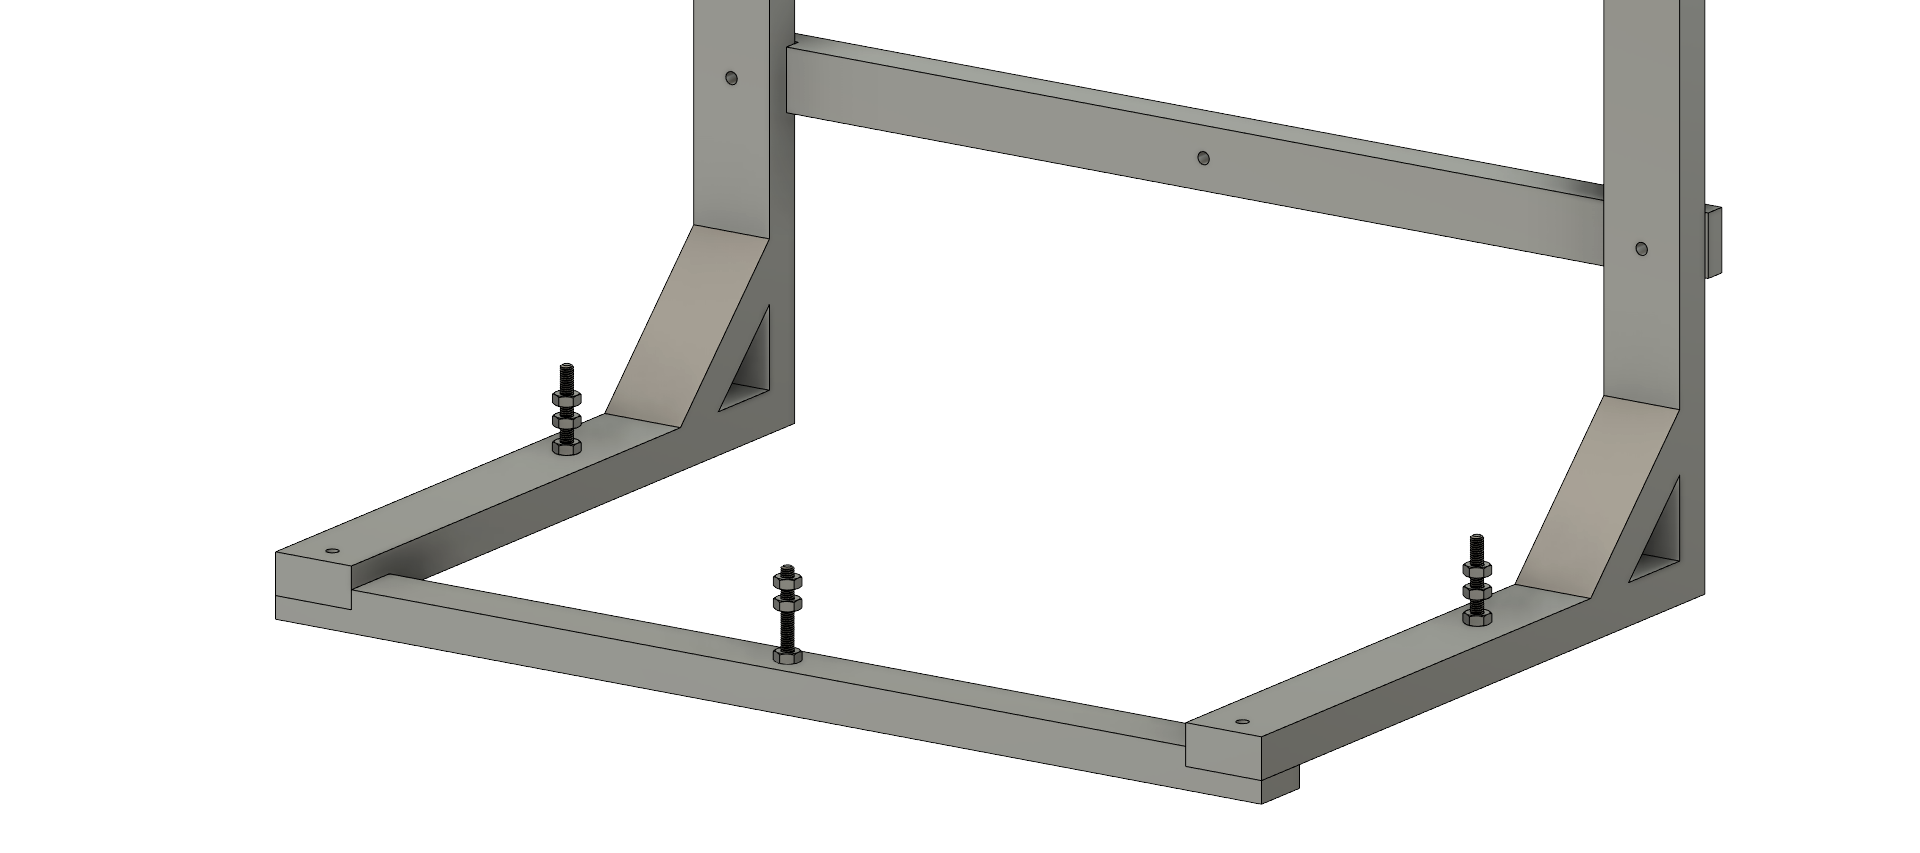
\includegraphics[width=12cm]{image/montage/boussole_solaire/6.png} 
\caption{Boulons servant de support au cadran d'azimut, modélisation 3D}
\end{figure}
~\\
Le cadran d'azimut est imprimé sur du papier ordinaire puis plastifié pour résister aux intempéries, il est fixé sur la plaque de plexiglas grâce à huit aimants qui permettent de faire coïncider les bords pour être parallèle avec la plaque de plexiglas et donc indirectement avec la barre transversale du CM121.\\

\begin{figure}[H]
\centering
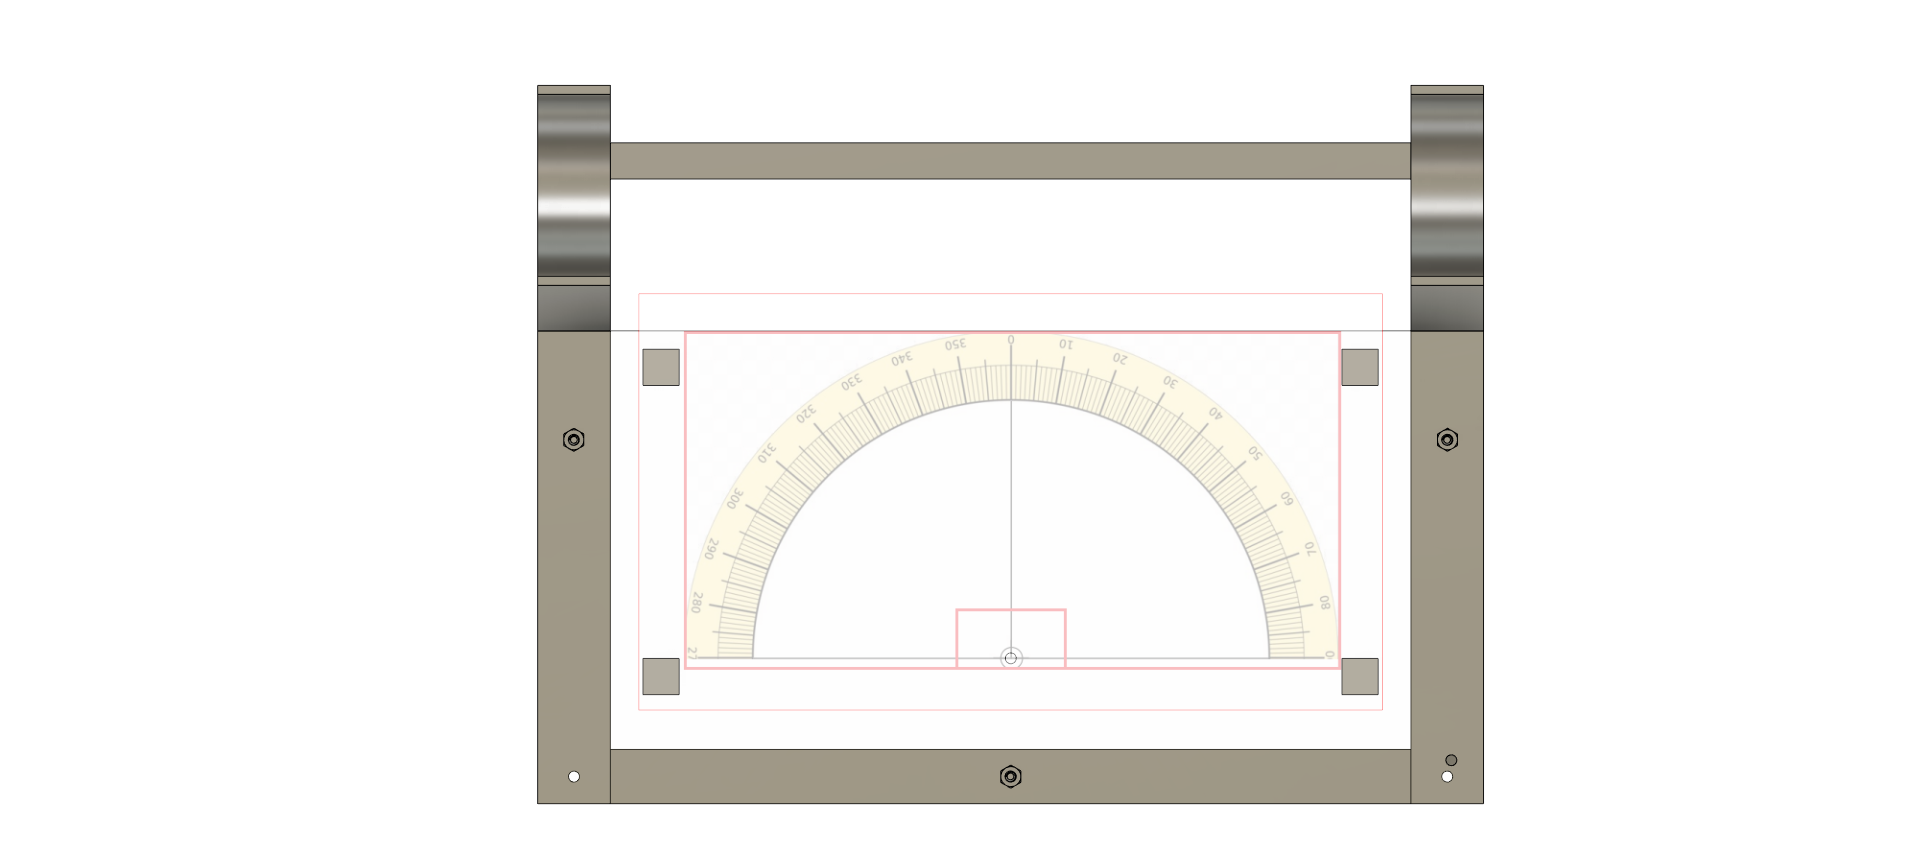
\includegraphics[width=12cm]{image/montage/boussole_solaire/5.png} 
\caption{Cadran d'azimut fixé par huit aimants, modélisation 3D}
\end{figure}

~\\
Vient ensuite la mise en place de la tige filetée de 3 mm qui supporte le fil. Le fil passe dans l'intersection du cadran d'azimut et la plaque de plexiglas par un trou de 3 mm, cela permet de réduire les effets du vent sur l'oscillation du fil.\\

 \begin{figure}[H]
\centering
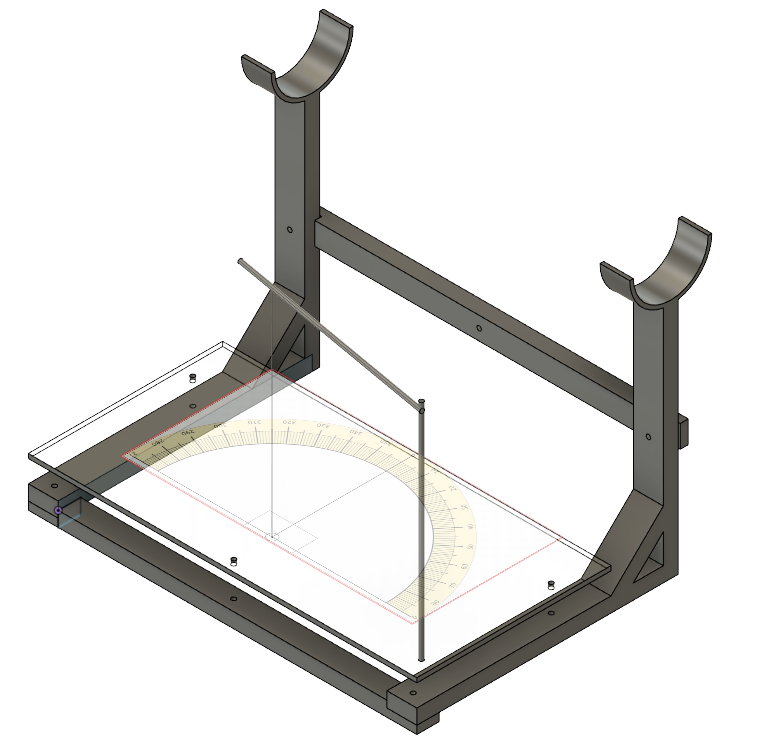
\includegraphics[width=8cm]{image/montage/boussole_solaire/1.png} 
\caption{Boussole solaire installée sur le CM121, modélisation 3D}  
\end{figure}
~\\
Le cadran est par la suite fixé à la barre transversale à l'aide de Colliers rilsan.

 \begin{figure}[H]
\centering
\includegraphics[width=6cm]{image/montage/boussole_solaire/8.jpg} 
\caption{Boussole solaire montée sur la barre transversale du CM121 }  
\end{figure}
~\\
La plaque de plexiglas doit ensuite être réglée à l'horizontale, pour se faire un niveau de surface est utilisé et les ajustements se font par les trois boulons de 3*30mm.


 \begin{figure}[H]
\centering
\includegraphics[width=6cm, angle=-90]{image/montage/boussole_solaire/7.jpg} 
\caption{Plaque de plexiglas de la boussole solaire réglée à l'horizontale}
\end{figure}
~\\
Nous devons maintenant connaître l'azimut du soleil, la solution la plus simple est d'utiliser un site internet via notre smartphone comme par exemple suncalc.org. L'azimut obtenu doit ensuite être reporté sur le cadran, pour ce faire, il suffit de faire pivoter la base du CM121 sur son axe vertical. Le positionnement nord-sud est effectué.\\
Cette méthode comporte quand même des limites, elle ne marche que pour les jours ensoleillés et la présence de masques cachent à certains moments de la journée le soleil ce qui empêche le positionnement nord-sud, mais le CM121 sera, à l'avenir, déplacé sur une plateforme ou il n'y aura aucun masque.  
 

\subsection{Programmation}

J'ai dû développer lors du stage des programmes en python permettant de calculer le calendrier pour le réglage du CM121, mais aussi d'effectuer l'analyse statistique d'une série de mesures. Pour ce faire mes programmes permettant d'effectuer l'analyse statistique fonctionnent avec des dataframes, j'ai porté mon choix vers les dataframes, car elles sont simples à manipuler.\\
~\\
Tous les programmes développés sont disponibles sur le \href{https://github.com/LE2P/pyranometre\_arc\_ombrage}{github du LE2P} [6].

\subsubsection{Calendrier du CM121}

Avant le stage, le réglage du CM121 se faisait de manière visuelle, il n'y avait pas de réglages précis à suivre. L'une de mes missions était le développement d'un calendrier pour le réglage du CM121. Sur ce calendrier devait figurer, les réglages pour chaque jour de l'année, les réglages minimums devant être effectués et l'heure du midi solaire qui sert entre autres à vérifier l'alignement nord-sud sur la boussole solaire fixe, si l'ombre au midi solaire indique 0°, alors l'alignement est effectif.\\
~\\
Le réglage de la barre coulissante est calculé en fonction de la déclinaison du soleil par l'expression (1): 

\begin{flalign}
&L = 297 tan (\delta)&&
\end{flalign}
Avec :\\
L : la position de la barre coulissante\\
$\delta$ : la déclinaison du soleil\\
~~\\
Nous pouvons retrouver cette équation en calculant le côté opposé à l'angle aigu d'un triangle rectangle, comme sur la figure suivante :

\begin{figure}[H]
\centering
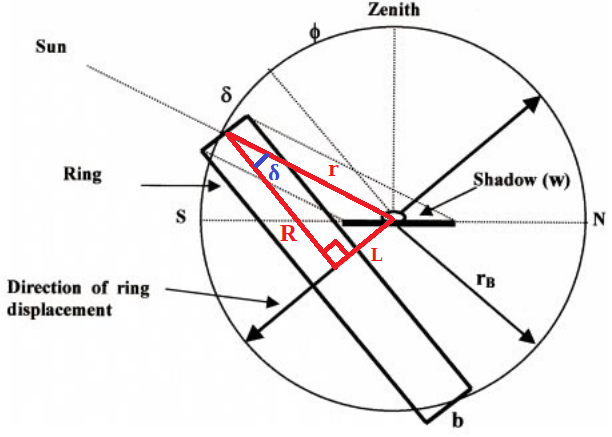
\includegraphics[width=8cm]{image/calendrier/1.PNG} 
\caption{Représentation géométrique du CM121}
\caption*{source :\href{https://journals.ametsoc.org/view/journals/atot/19/5/1520-0426_2002_019_0698_ansrdf_2_0_co_2.xml}{https://journals.ametsoc.org}} 
\end{figure}

\begin{flalign}
&tan(\delta) = \frac{L}{R}&&\\
&L = R~tan(\delta)&&\\
&L = 297tan(\delta)&&
\end{flalign}
~~\\
Le programme calcule aussi les maintenances minimums à effectuer en se basant sur la déclinaison du soleil. Étant donné que la position de la barre coulissante est obtenue en fonction de la déclinaison, nous pouvons calculer les jours de réglage minimum au cours de l'année. Pour ce faire, on place la barre coulissante pour le jour correspondant (la position normale), puis nous déplaçons la barre pour obtenir l'ombre à 0.5 mm du dôme en verre du pyranomètre (la position limite).

\begin{figure}[H]
    \begin{minipage}[c]{.46\linewidth}
        \centering
        \includegraphics[width=8cm]{image/calendrier/6.jpg} 
        \caption{Position normale de la barre coulissante du CM121}
    \end{minipage}
    \hfill%
    \begin{minipage}[c]{.46\linewidth}
        \centering
        \includegraphics[width=8cm]{image/calendrier/5.jpg} 
        \caption{Position limite de la barre coulissante du CM121}
    \end{minipage}
\end{figure}

~~\\
Il suffit maintenant de savoir la déclinaison pour la position normale et la position limite, pour obtenir la déclinaison de la position limite, il nous suffit de lire la position de la barre coulissante et de regarder sur notre calendrier de maintenance le jour correspondant, il nous suffit maintenant de calculer la déclinaison pour ce jour. On peut désormais calculer la différence des déclinaisons.\\

\begin{flalign}
&\Delta \delta=\delta_{position~normale}-\delta_{position~limite}&&\\
&\Delta \delta=1.3^\circ&&
\end{flalign}
~\\
Nous trouvons une différence de 1.3°, cela signifie que si la déclinaison subit une variation de $\pm 1.3^\circ$  entre la dernière maintenance et aujourd'hui, nous devons effectuer le réglage de la barre coulissante.\\
~\\
Le programme retourne alors trois calendriers, un calendrier au format CSV, un calendrier au format XLSX et un calendrier ICS. \\
~\\
Le calendrier CSV est obtenu par du texte brut ce qui signifie qu'il fonctionne avec tous les logiciels de traitement de texte, mais ce format ne permet pas la mise en forme. \\
~\\
Le calendrier XLSX permet d'intégrer la mise en forme au calendrier, nous obtenons ainsi des codes couleurs, en vert les jours fériés, en bleu les week-ends et en rouge les maintenances minimums à effectuer sur le CM121. \\
~\\
Le calendrier ICS permet d'avoir les positions du CM121 au format iCalendar ce qui permet entre autres d'avoir le midi-solaire, la position de la barre coulissante et les maintenances minimums via son smartphone par des notifications, cela offre une souplesse d'utilisation comparée aux deux autres calendriers.\\

\begin{figure}[H]
\centering
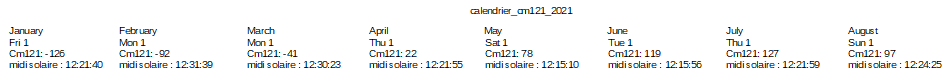
\includegraphics[width=16cm]{image/calendrier/3.PNG} 
\caption{Calendrier de réglage du CM121 au format CSV}  
\end{figure}

\begin{figure}[H]
\centering
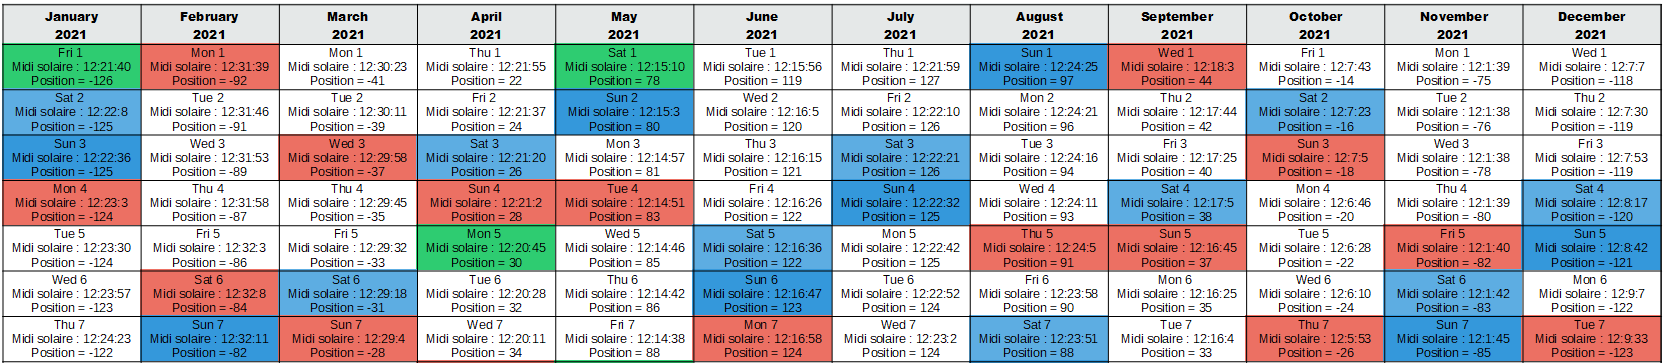
\includegraphics[width=16cm]{image/calendrier/2.PNG} 
\caption{Calendrier de réglage du CM121 au format XLSX}  
\end{figure}


\begin{figure}[H]
    \begin{minipage}[c]{.46\linewidth}
        \centering
        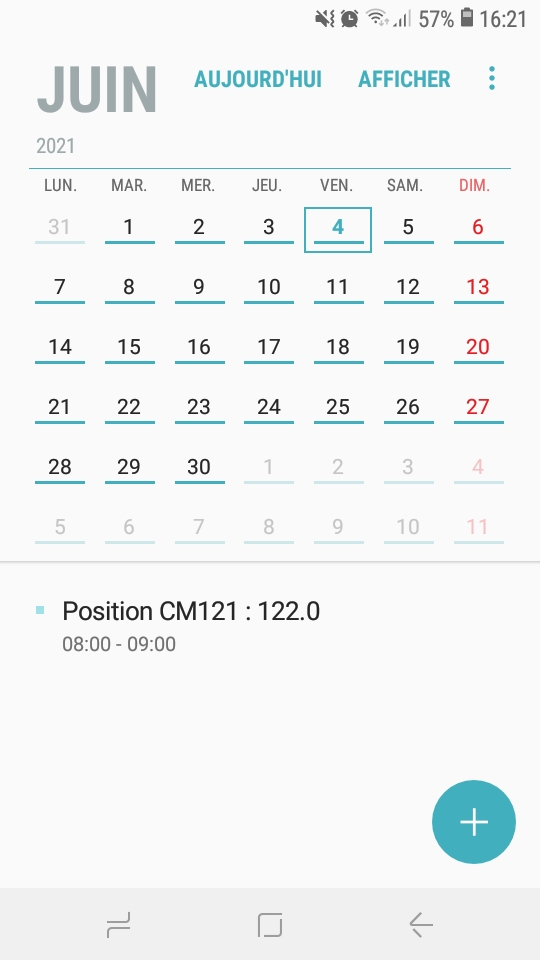
\includegraphics[width=5cm]{image/calendrier/4.jpg} 
		\caption{Calendrier de réglage du CM121 au format ICS}
    \end{minipage}
    \hfill%
    \begin{minipage}[c]{.46\linewidth}
        \centering
        \includegraphics[width=5cm]{image/calendrier/7.jpg} 
        \caption{Calendrier de réglage du CM121 au format ICS avec notification de réglage minimum}
    \end{minipage}
\end{figure}

\subsubsection{Suppression des données non utilisées, non acquises et aberrantes}

~\\
Les fichiers de mesures comportent généralement des données erronées que ce soit pour le CM121, le SPN1 ou le tracker. Ces données peuvent bloquer l'exécution de certains programmes, ces données sont repérées sous Python, car elles ont pour valeur "Nan", "inf" et "-inf". Les fichiers de mesures comportent aussi les données pour la nuit qui sont inintéressantes pour l'étude du rayonnement solaire, la création d'une fonction pour supprimer ces mesures fut nécessaire. Elle consiste à repérer ces valeurs et à supprimer les lignes correspondantes.

\subsubsection{Calcul des facteurs de correction}

Les mesures du CM121 doivent être corrigées, car l'arc d'ombrage masque une partie du diffus. L'expression permettant de calculer le facteur de correction donné par le fabricant du CM121 se base sur les travaux de Drummond. Cette correction fait l'hypothèse que le rayonnement diffus est isotrope ce qui donne une correction des mesures purement géométrique.\\
~\\
Les mesures du CM121 sont corrigées par une fonction qui calcule les facteurs de correction en se basant sur l'heure ou les mesures ont été prises, ils sont appliqués par la suite aux mesures.

\subsubsection{Analyse statistique et étalonnage}

Le capteur du pyranomètre possède une sensitivité qui change à travers le temps, de ce fait le pyranomètre doit subir un étalonnage. 

\begin{figure}[H]
\centering
\includegraphics[width=5cm]{image/etallonnage/20210416_093654.jpg} 
\caption{Sensitivité du pyranomètre}  
\end{figure}
~\\
La nouvelle sensibilité peut être déterminée en comparant nos mesures avec les mesures d'un pyranomètre de référence, elle est obtenue par la relation :

\begin{flalign}
&DHI_{mesure}=a.DHI_{r\acute{e}f\acute{e}rence} &&\\
&\frac{U}{S_{mesure}} =a. \frac{U}{S_{r\acute{e}f\acute{e}rence}}&&\\
&S_{mesure}.a = S_{r\acute{e}f\acute{e}rence}&&
\end{flalign}
~\\
Pour obtenir la nouvelle sensibilité de notre pyranomètre nous devons alors calculer le coefficient 'a', pour obtenir ce coefficient nous réalisons une régression linéaire. Nous obtenons alors une droite d'équation $y = ax + b$ ou 'b' est négligé.\\
~\\
La fonction développée permet d'effectuer l'étalonnage, mais aussi l'analyse statistique. L'analyse statistique permet d'obtenir sur le graphique le coefficient de détermination $R^2$, la variance, l'erreur quadratique moyenne et l'erreur absolue moyenne.\\
~\\
Le coefficient de détermination ($R^2$) est un indicateur qui permet de juger la qualité d’une régression linéaire. Si le $R^2$ vaut 1, cela signifie que l’équation de la droite de régression est capable de déterminer 100 \% de la distribution des points. Cela signifie alors que le modèle mathématique utilisé, ainsi que les paramètres "a" et "b" calculés sont ceux qui déterminent la distribution des points.\\
~~\\
La variance ($\sigma ^2$) permet de mesurer la dispersion des valeurs d'un échantillon, plus elle est élevée, plus la dispersion est élevée. On définit la variance d'une variable discrète composée de n observations comme suit :\\

\begin{flalign}
&\sigma ^2 =  \frac{\sum(X+\overline{X})^2}{n}&&\\
& \overline{X} : moyenne&&\\
& X : valeur incluse dans l'ensemble des données&&
\end{flalign}

~~\\
L'erreur quadratique moyenne (RMSE) fournit une indication par rapport à la dispersion ou la variabilité de la qualité de la prédiction, il est souvent relié à la variance, car les valeurs de RMSE sont difficiles à interpréter parce que l’on n'est pas en mesure de dire si on a une variance faible ou forte, l'erreur quadratique moyenne donne plus de poids aux erreurs élevés. On définit l'erreur quadratique moyenne comme par :

\begin{flalign}
&RMSE = \sqrt{\frac{1}{N}  \overset{N}{\underset{i=1}{\sum}} (\widehat{y}_i -y_i)^2 }&&
\end{flalign}
~\\ 
L'erreur absolue moyenne (MAE) représente l'erreur systématique, toutes les différences individuelles ont le même poids.\\

\begin{flalign}
&MAE = \frac{1}{N}  \overset{N}{\underset{i=1}{\sum}} |\widehat{y}_i -y_i| &&
\end{flalign}


~\\
La fonction renvoie les graphiques avant étalonnage et après étalonnage, avec en rouge une densité de points élevés et en bleu une densité de point faible.
\begin{figure}[H]
\centering
\includegraphics[width=15cm]{image/etallonnage/2.png} 
\caption{Mesure sans étalonnage du CM121 pour mars 2021}  
\end{figure}

\begin{figure}[H]
\centering
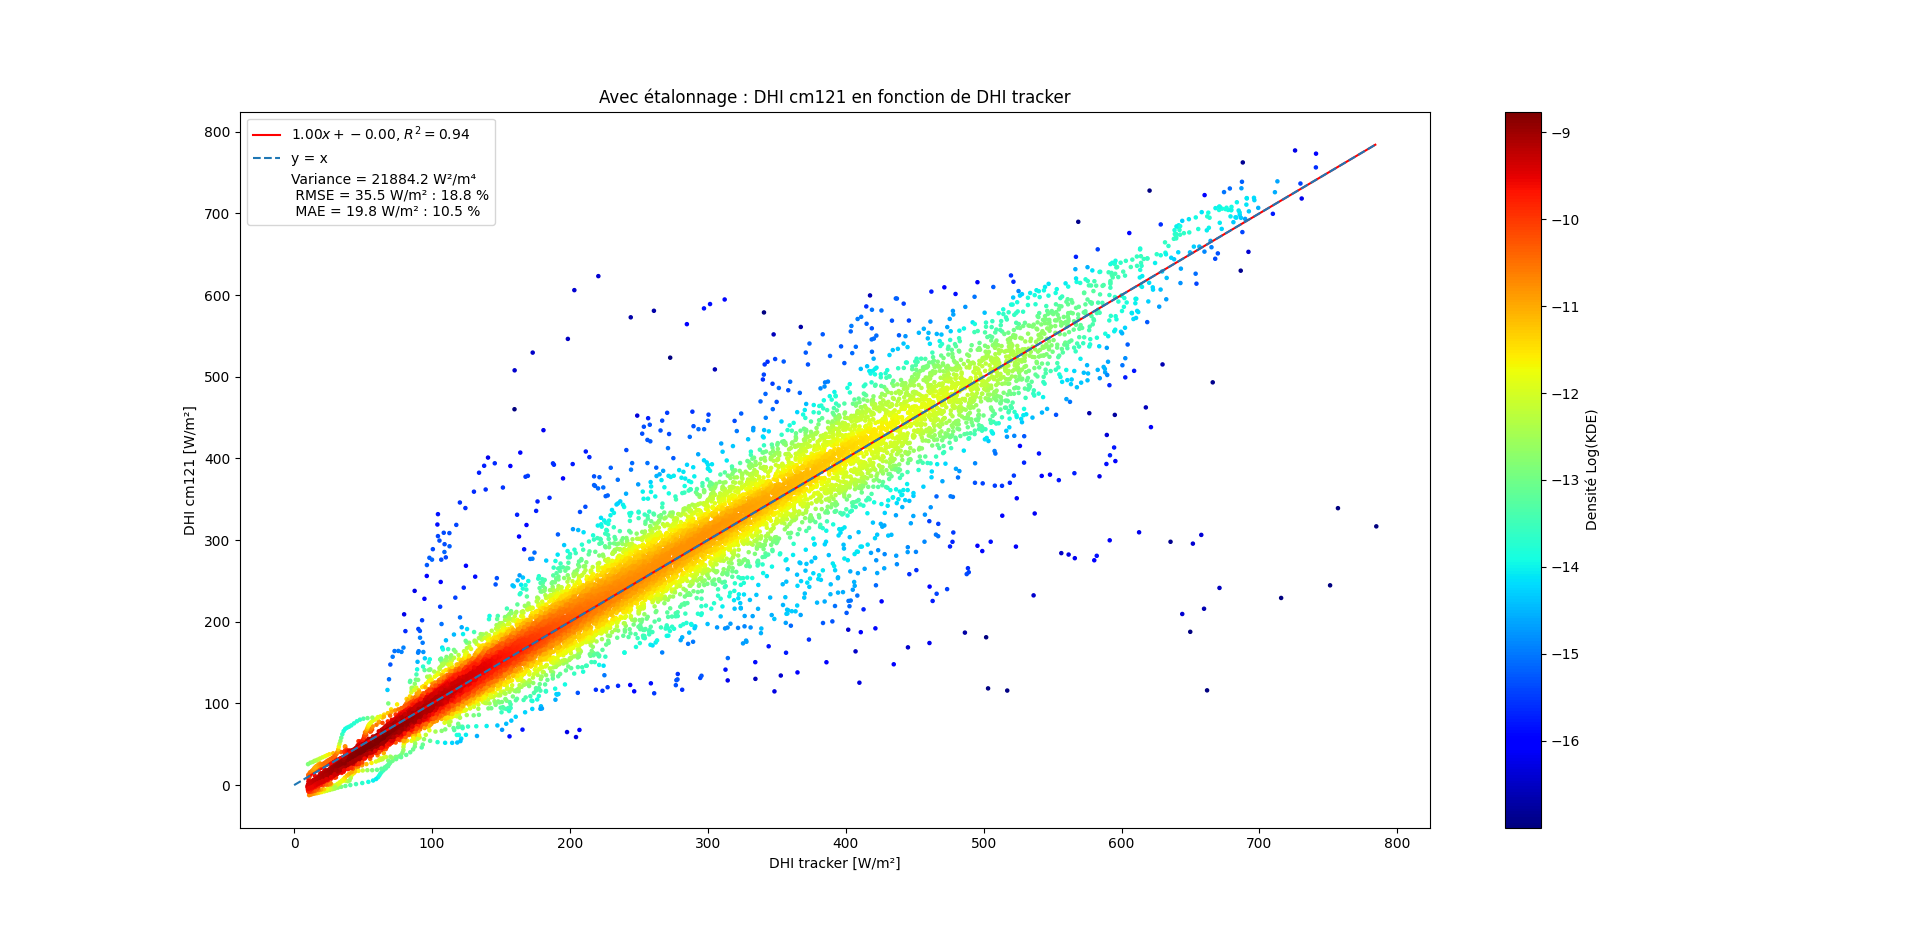
\includegraphics[width=15cm]{image/etallonnage/1.png} 
\caption{Mesure avec étalonnage du CM121 pour mars 2021}  
\end{figure}


\subsubsection{Représentation graphique de l'erreur relative}

L'erreur relative $\delta \alpha_r$ est obtenue par :
\begin{flalign}
&\delta \alpha_r = \frac{valeur~mesur\acute{e}e-valeur~r\acute{e}f\acute{e}rence}{|valeur~r\acute{e}f\acute{e}rence|} &&
\end{flalign}
~\\
Il est intéressant d'avoir la représentation de l'erreur relative en fonction de l'azimut et de l'élévation du soleil, cela permet de mettre en lumière des journées particulières comme par exemple le dysfonctionnement de l'acquisition des mesures, mais aussi la présence de masques ou de reflet impactant le pyranomètre. Les erreurs aberrantes qui sont identifiées grâce à cette méthode peuvent donc être supprimées.\\
~\\
La fonction développée renvoie le graphique ci-dessous, nous constatons des erreurs relatives élevées pour le lever et le coucher du soleil, mais aussi durant certaines journées.
 
\begin{figure}[H]
\centering
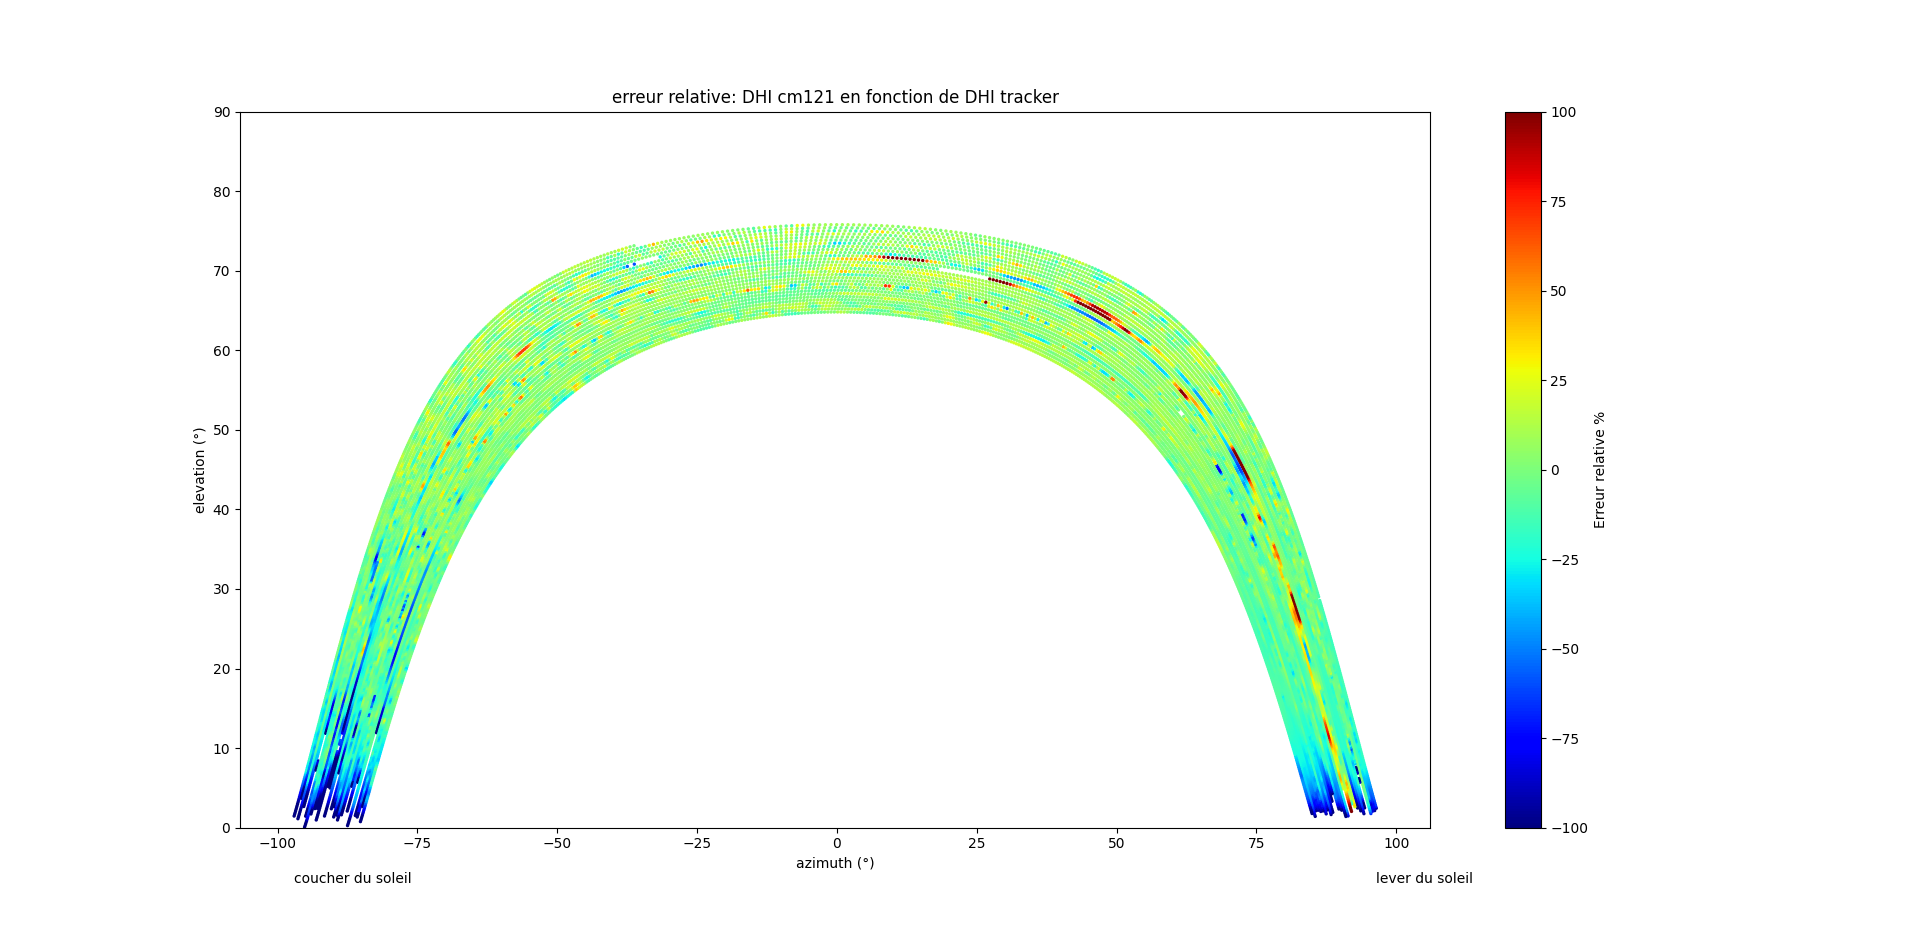
\includegraphics[width=15cm]{image/erreur_relative/1.png} 
\caption{Représentation de l'erreur relative du CM121 en fonction du tracker pour mars 2021}  
\end{figure}

\subsubsection{Histogramme}

La dernière fonction pour l'analyse statistique est l'histogramme, il donne la représentation graphique de la répartition d'une variable, dans notre cas la fonction donne la répartition du rayonnement diffus et de l'erreur relative. C'est une information supplémentaire, elle nous permet de savoir si le ciel pour la période souhaitée était plutôt dégagé ou nuageux, mais aussi, si l'acquisition des mesures était bonne, dans ce cas la répartition des erreurs relative serait majoritairement centrée sur le zéro.\\
Elle renvoie les graphiques ci-dessous.
\begin{figure}[H]
\centering
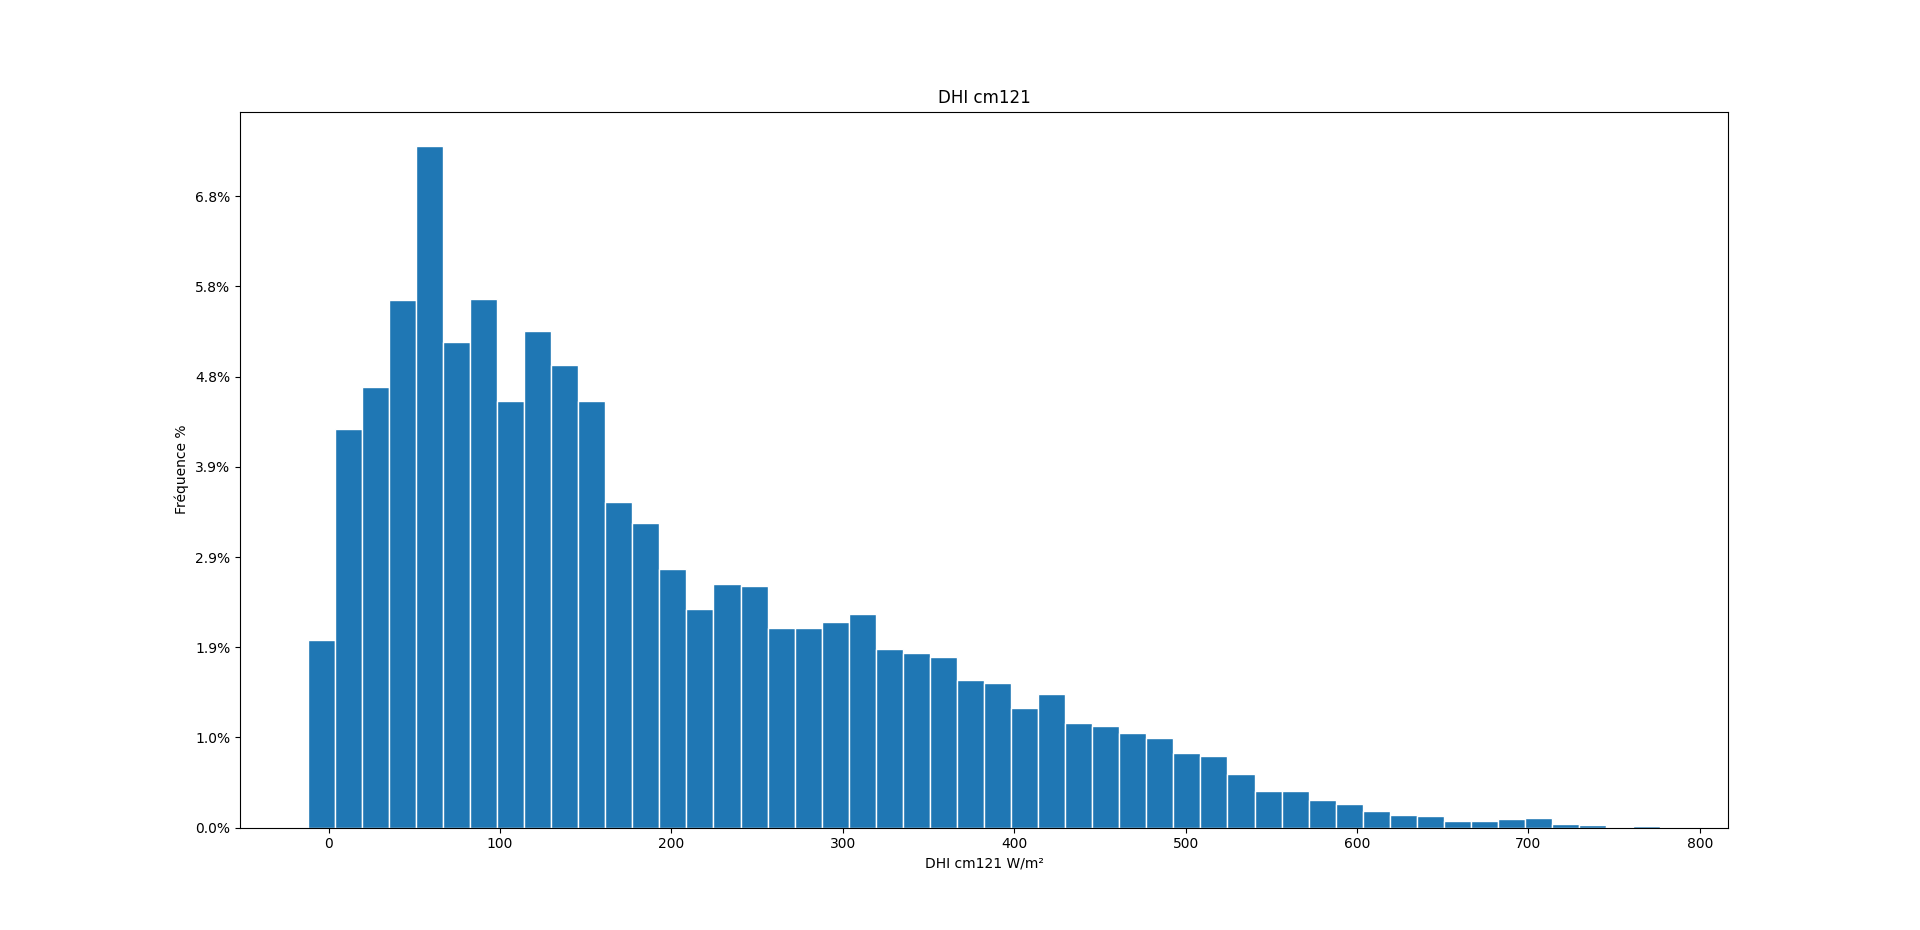
\includegraphics[width=15cm]{image/histogramme/1.png} 
\caption{Répartition du rayonnement diffus du CM121 pour mars 2021}  
\end{figure}

\begin{figure}[H]
\centering
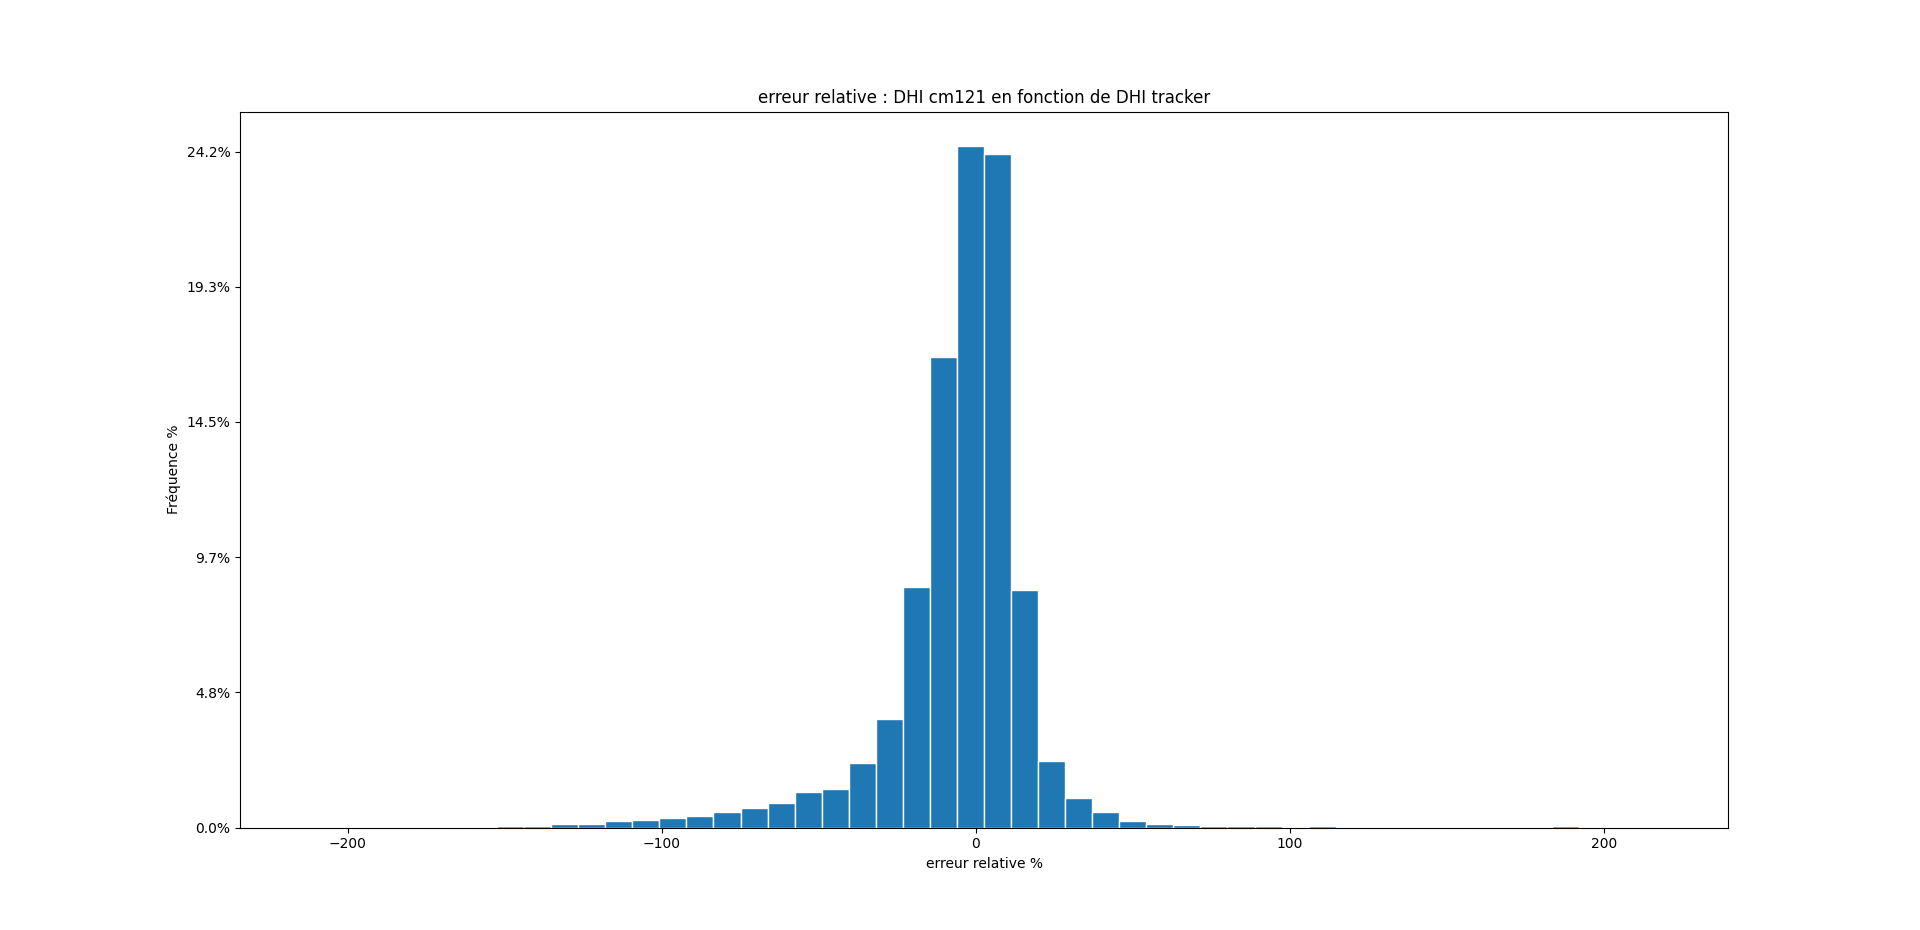
\includegraphics[width=15cm]{image/histogramme/2.png}  
\caption{Répartition de l'erreur relative du rayonnement diffus du CM121 en fonction du tracker pour mars 2021}  
\end{figure}


\subsubsection{Sélection des mesures entre deux intervalles}

Deux fonctions ont été créées permettant de sélectionner les mesures pour une période donnée, la première permet d'avoir les mesures entre deux dates et la dernière permet d'avoir les mesures pour une tranche horaire spécifiée. Après la sélection de la période souhaitée, l'opérateur lance l'analyse statistique.

\subsubsection{Exécution de l'analyse statistique}

Pour faciliter l'utilisation du programme celui-ci s'exécute via un terminal, pour ce faire l'utilisateur doit juste renseigner le nom de son fichier de mesure, choisir les valeurs pour la mesure, la référence et lancer l'analyse. Si l'utilisateur le souhaite, il est aussi en mesure de renseigner la période sur laquelle il souhaite l'analyse statistique que ce soit entre deux dates, une tranche horaire ou entre deux dates pour une tranche horaire.


\subsubsection{Comparaison du CM121 avec le SPN1 et le tracker}

Le CM121 et le SPN1 utilise tous deux un arc pour masquer le rayonnement direct du soleil, cet arc donne un angle de vue de 10.8° pour le CM121 et le SPN1, alors que le masque du tracker une sphère qui donne un angle de vue de 5°. Nous cherchons donc à déterminer si les mesures du CM121 sont plus proches du SPN1 que du tracker de part sa conception.

\begin{figure}[H]
    \begin{minipage}[c]{.2\linewidth}
        \centering
        \includegraphics[width=5cm]{image/presentation_cm121/2.jpg}  

    \end{minipage}
    \hfill%
    \begin{minipage}[c]{.2\linewidth}
        \centering
        \includegraphics[width=5cm]{image/presentation_cm121/3.jpg}  

    \end{minipage}
    \hfill%
    \begin{minipage}[c]{.3\linewidth}
        \centering
        \includegraphics[width=5cm]{image/presentation_cm121/4.jpg} 

    \end{minipage}
    \caption{CM121, tracker et SPN1 sur la plateforme de la Faculté des Sciences et Technologies, Université de la Réunion Campus du Moufia}
\end{figure}
~\\
L'analyse statistique est effectuée entre le 01 janvier 2021 jusqu'au 01 avril 2021, elle est réalisée une première fois globalement, puis pour les données entre 5h et 12h et enfin entre 12h et 19h. Les graphiques obtenus sont disponibles en annexe (annexe 1 à 3).
~\\



\begin{table}[H]
\begin{center}
\begin{tabular}{ |c|c|c|c|c| } 
 \hline
  & $R^2$ & $\sigma ^2 [\frac{W^2}{m^4}]$ & RMSE [\%] & MAE [\%] \\ 
  \hline
  \multicolumn{5}{|c|}{Globale} \\
  \hline
 CM121 vs tracker & 0.96 & 23992.6 & 17.7 & 9.7\\ 
 \hline
 CM121 vs SPN1 & 0.97 & 24047.3 & 15.1 & 8.6 \\ 
 \hline
  \multicolumn{5}{|c|}{Entre 5h et 12h} \\
  \hline
   CM121 vs tracker & 0.95 & 20373.1 & 20.5 & 10.2\\ 
 \hline
 CM121 vs SPN1 & 0.96 & 20753 & 17.4 & 9.3 \\
 \hline
  \multicolumn{5}{|c|}{Entre 12h et 19h} \\
  \hline 
   CM121 vs tracker & 0.96 & 25979.3 & 16 & 9.5\\ 
 \hline
 CM121 vs SPN1 & 0.97 & 25810.8 & 13.5 & 8 \\
 \hline
\end{tabular}
\caption{Indicateur statistique CM121 vs tracker et CM121 vs SPN1}
\end{center}
\end{table}

~\\
De manière globale, que ce soit le matin ou l'après-midi, on constate que les variances sont très proches, qui plus en comparant le CM121 avec le SPN1 les erreurs quadratiques moyennes et les erreurs absolues moyennes sont plus faibles et les coefficients de détermination sont plus élevés. Les mesures du CM121 sont donc plus proches des mesures du SPN1 que ceux du tracker, de part sa conception. \\



\subsubsection{Impact de la ventilation sur les mesures du CM121}

Les mesures avec la ventilation opérationnelle ont été acquise entre le 21 avril 2021 et le 31 mai 2021, nous devons donc comparer les mesures avec ventilation et sans ventilation sur une même période de 41 jours, les mesures entre le 21 avril 2021 et le 31 mai 2021 (avec ventilation) sont comparées aux mesures entre le 11 mars et le 20 avril (sans ventilation).

\begin{figure}[H]
\centering
\includegraphics[width=12cm]{image/impact_ventillation/archive_2021-03-11_2021-04-20/regression_avec_étalonnage_DHI cm121vsDHI tracker.png}  
\caption{CM121 en fonction du tracker sans ventilation}  
\end{figure}

\begin{figure}[H]
\centering
\includegraphics[width=12cm]{image/impact_ventillation/avril_mai_2021/regression_avec_étalonnage_DHI cm121vsDHI tracker.png} 
\caption{CM121 en fonction du tracker avec ventilation}  
\end{figure}



\begin{figure}[H]
\centering
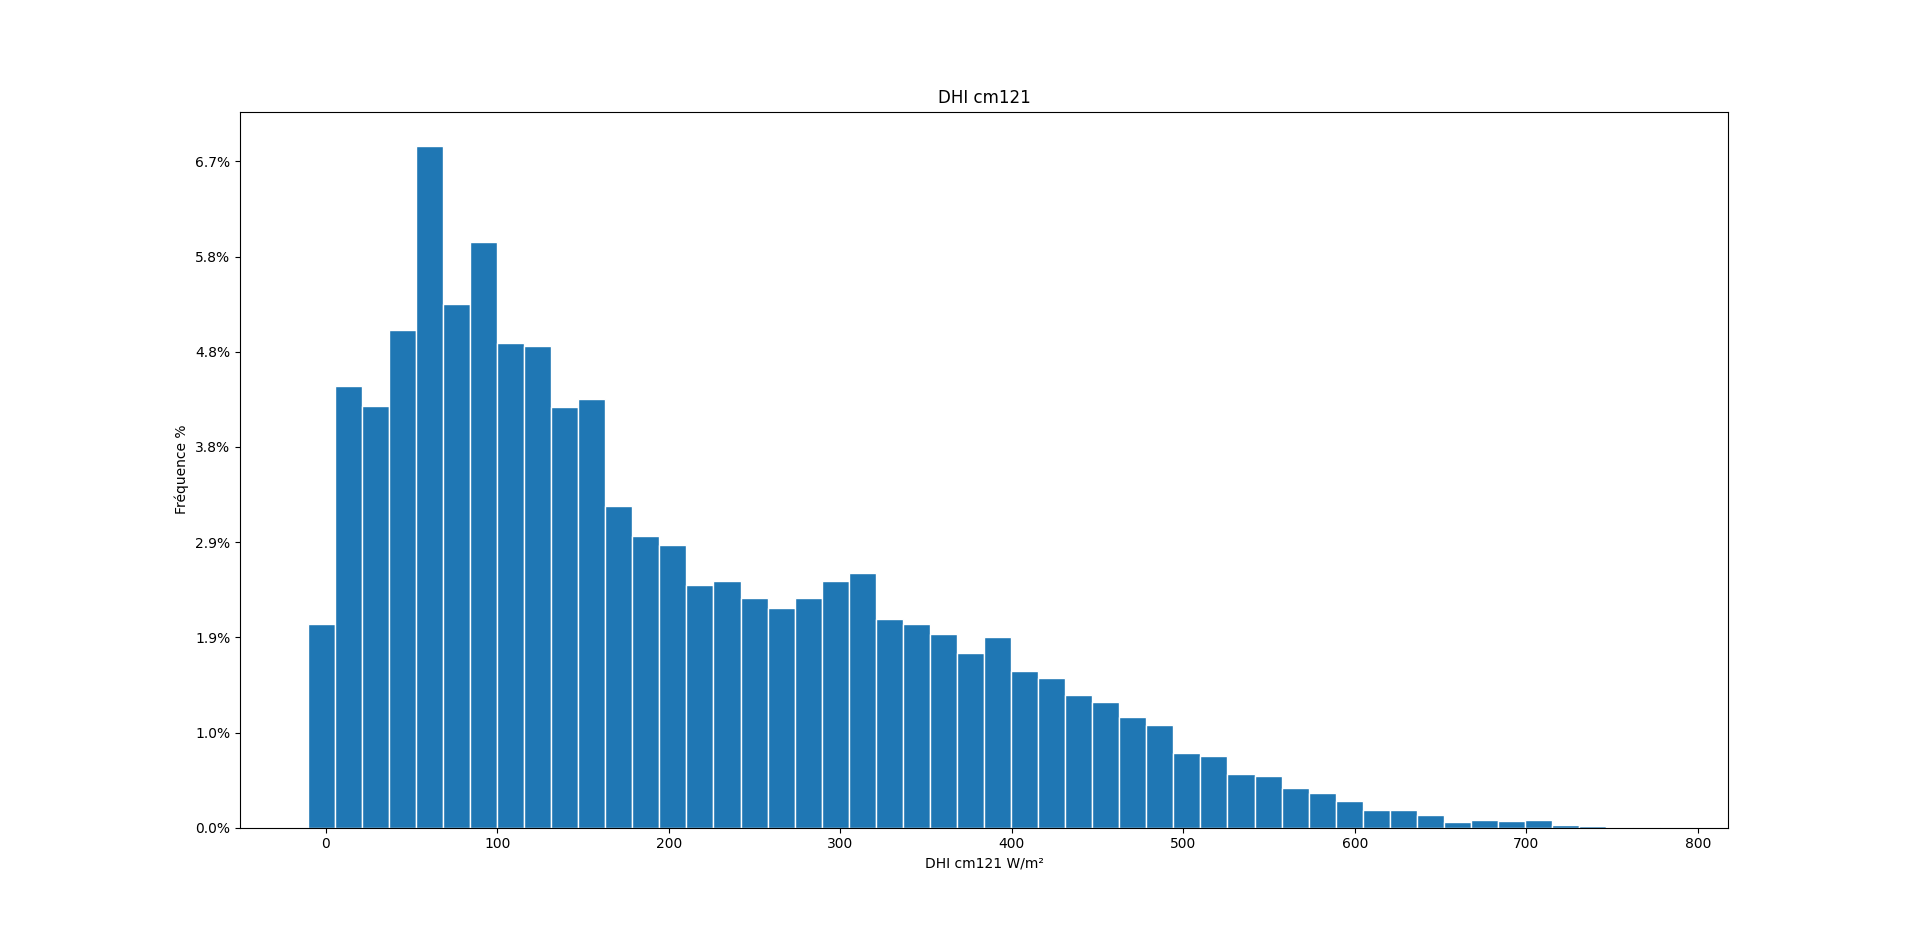
\includegraphics[width=15cm]{image/impact_ventillation/archive_2021-03-11_2021-04-20/histogramme_3.png} 
\caption{Répartition du DHI sans ventilation}  
\end{figure}

\begin{figure}[H]
\centering
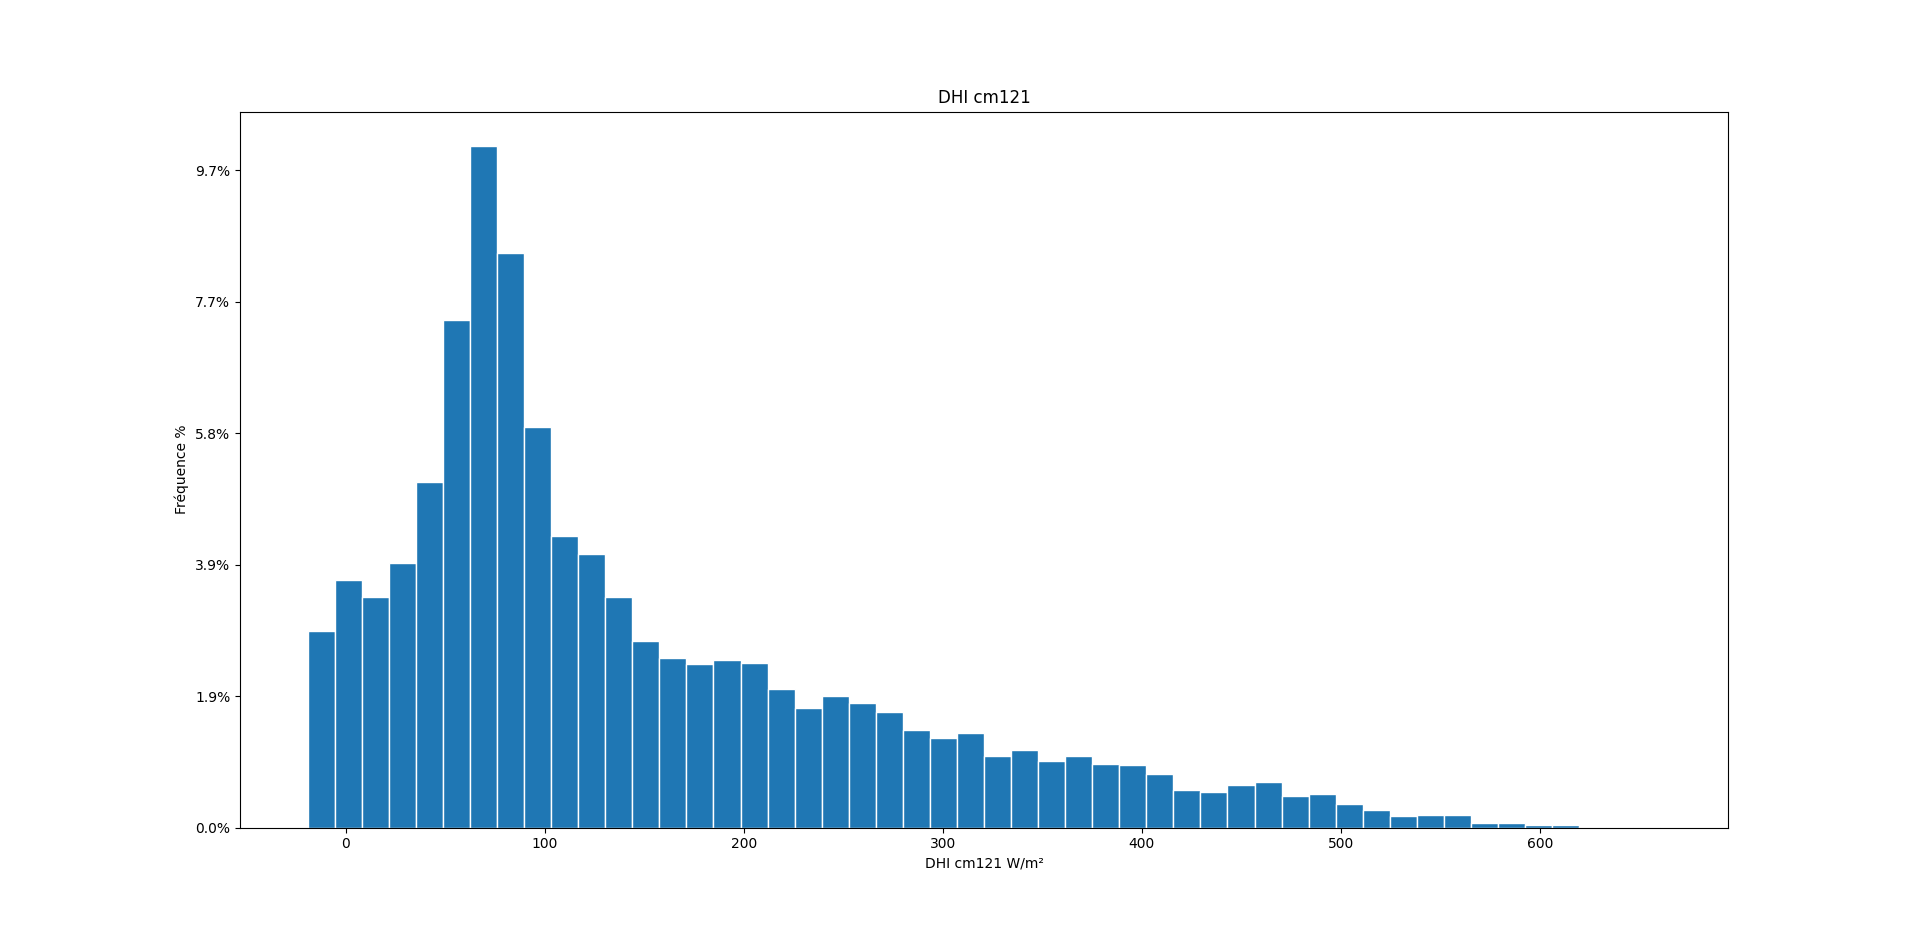
\includegraphics[width=15cm]{image/impact_ventillation/avril_mai_2021/histogramme_3.png}  
\caption{Répartition du DHI avec ventilation}  
\end{figure}




\begin{table}[H]
\begin{center}
\begin{tabular}{ |c|c|c|c|c| } 
 \hline
  & $R^2$ & $\sigma ^2 [\frac{W^2}{m^4}]$ & RMSE [\%] & MAE [\%] \\ 
  \hline
 Avec ventilation & 0.86 & 15741.5 & 31.8 & 14.4\\ 
 \hline
 Sans ventilation & 0.95 & 22587.1 & 16.3 & 9.2 \\ 
 \hline
\end{tabular}
\caption{Indicateurs statistiques pour l'impact de la ventilation sur les mesures du CM121}
\end{center}
\end{table}

~\\
Les histogrammes nous montrent que pour les deux périodes la répartition du rayonnement diffus est similaire.
Nous obtenons avec la mise en place de la ventilation une erreur quadratique moyenne et une erreur absolue moyenne plus élevé, en revanche la variance est plus faible, les mesures ont donc moins de dispersion avec la ventilation. Dire que la ventilation augmente l'erreur quadratique moyenne et l'erreur absolue moyenne semble fausse, pour obtenir des résultats plus concrets, il faudrait réaliser la même étude sur une période plus longue. Les résultats peuvent venir du fait que la période d'acquisition était particulière.

\subsection{Les apports du stage}

Le stage m'a permis de découvrir le langage de programmation Python, ainsi que l'utilisation de github qui permet d'enregistrer les différentes versions de son projet, mais aussi les bonnes pratiques que ce soit pour la programmation ou l'organisation de son répertoire de travail. J'ai également pu apprendre l'utilisation d'un logiciel de modélisation 3D, fusion 360, ainsi que le principe de la boussole solaire. Il m'a aussi permis de mettre en place les outils nécessaires et leur choix dans le cas de l'analyse statistique.


\section{Conclusion}

Les missions demandées lors du stage firent mener à bien, que ce soit le calendrier de réglage du CM121, la mise en place d'un dispositif permettant un réglage précis et simple de la position nord-sud, ou encore le développement de programme sous Python permettant l'analyse statistique d'un jeu de données.\\
~\\
Le stage a permis de mettre en lumière que les mesures du CM121 sont plus proches du SPN1 que du tracker, l'étude statistique a montré une variance similaire dans le cas où le CM121 est comparé au tracker et dans le cas où le CM121 est comparé au SPN1, ce qui signifie que dans les deux cas la dispersion des mesures est la même. La comparaison avec le SPN1 donne les erreurs quadratiques moyennes et les erreurs absolues moyennes les plus faibles, ce qui montre que les mesures ont moins d'erreurs élevées et systématiques, les mesures du CM121 sont donc plus proche du SPN1 que du tracker.\\
~\\
Le stage a aussi montré que la ventilation permet d'avoir moins de dispersion, mais paradoxalement, elle donne une erreur quadratique moyenne et une erreur absolue moyenne plus élevé, divers facteurs peuvent expliquer cela comme notamment une période d'acquisition trop courte, pour valider ce résultat, il semble judicieux de refaire cette analyse statistique dans le futur avec une période d'acquisition plus longue.

\newpage

\section{Bibliographie}


$[1]$ The assessment of four different correction models applied to the diffuse radiation measured with a shadow ring using global and normal beam radiation measurements for Beer Sheva, Israel. (2008). Solar Energy, [online] 82(2), pp.144–156. Available at: \url{https://www.sciencedirect.com/science/article/abs/pii/S0038092X07001338} [Accessed 5 Jun. 2021].\\
~\\
‌
$[2]$ Sánchez, G., Serrano, A. and Cancillo, M.L. (2013). Shadow-band correction for diffuse ultraviolet radiation measurements. Journal of Geophysical Research: Atmospheres, 118(9), pp.3807–3816.\\

‌~\\
$[3]$ Shadow-band radiometer measurement of diffuse solar irradiance: Calculation of geometrical and total correction factors. (2016). Solar Energy, [online] 139, pp.85–99.\\ 
Available at: \url{https://www.sciencedirect.com/science/article/abs/pii/S0038092X16304327#:~:text=Taking\%20into\%20account\%20that\%20a} [Accessed 5 Jun. 2021].\\

‌~\\
$[4]$ On shadowband correction methods for diffuse irradiance measurements. (1995). Solar Energy, [online] 54(2), pp.105–114. Available at: \url{https://www.sciencedirect.com/science/article/abs/pii/0038092X9400115T} [Accessed 5 Jun. 2021].\\

‌~\\
$[5]$ A shadow-ring device for measuring diffuse solar radiation on a vertical surface in a tropical zone. (2016). Solar Energy, [online] 136, pp.629–638. Available at: \url{https://www.sciencedirect.com/science/article/abs/pii/S0038092X16303012#:~:text=A\%20shadow\%2Dring\%20device\%20is} [Accessed 5 Jun. 2021].\\
‌~\\
$[6]$ \url{https://github.com/LE2P/pyranometre\_arc\_ombrage} \\
~\\
$[7]$ \url{https://rratlas.energy.gov.sa/RRMMPublicPortal/sites/default/files/How\%20to\%20Read\%20Live\%20Graph.htm} \\
~\\
$[8]$JJ (2016). MAE and RMSE — Which Metric is Better? [online] Medium. Available at: \href{https://medium.com/human-in-a-machine-world/mae-and-rmse-which-metric-is-better-e60ac3bde13d}{https://medium.com/human-in-a-machine-world/mae-and-rmse-which-metric-is-better-e60ac3bde13d}\\
~\\
$[9]$ May, P.T., Cummings, F., Koutsovasilis, J., Jones, R. and Shaw, D. (2002). The Australian Bureau of Meteorology 1280-MHz Wind Profiler. Journal of Atmospheric and Oceanic Technology, [online] 19(6), pp.911–923. Available at: \url{https://journals.ametsoc.org/view/journals/atot/19/6/1520-0426_2002_019_0911_tabomm_2_0_co_2.xml}

\newpage

‌\section{Annexes}
\subsection*{Annexe 1}
Analyse statistique pour le 01 janvier 2021 jusqu'au 01 avril 2021.

\begin{figure}[H]
\centering
\includegraphics[width=15cm]{image/comparaison_cm121_spn1/cm121_tracker_2021-01-01_2021-04-01/regression_avec_étalonnage_DHI cm121vsDHI tracker.png} 
\caption{cm121 en fonction du tracker}    
\end{figure}

\begin{figure}[H]
\centering
\includegraphics[width=15cm]{image/comparaison_cm121_spn1/cm121_spn1_2021-01-01_2021-04-01/regression_avec_étalonnage_DHI cm121vsDHI spn1.png}  
\caption{cm121 en fonction du spn1} 
\end{figure}

\newpage

\subsection*{Annexe 2}
Analyse statistique pour le 01 janvier 2021 jusqu'au 01 avril 2021 de 5h à 12h.

\begin{figure}[H]
\centering
\includegraphics[width=15cm]{image/comparaison_cm121_spn1/cm121_tracker_5_00_00_12_00_00_2021-01-01_2021-04-01/regression_avec_étalonnage_DHI cm121vsDHI tracker.png}  
\caption{cm121 en fonction du tracker}
\end{figure}

\begin{figure}[H]
\centering
\includegraphics[width=15cm]{image/comparaison_cm121_spn1/cm121_spn1_5_00_00_12_00_00_2021-01-01_2021-04-01/regression_avec_étalonnage_DHI cm121vsDHI spn1.png}  
\caption{cm121 en fonction du spn1}  
\end{figure}

\newpage
\subsection*{Annexe 3}
Analyse statistique pour le 01 janvier 2021 jusqu'au 01 avril 2021 de 12h à 19h.


\begin{figure}[H]
\centering
\includegraphics[width=15cm]{image/comparaison_cm121_spn1/cm121_tracker_12_00_00_19_00_00_2021-01-01_2021-04-01/regression_avec_étalonnage_DHI cm121vsDHI tracker.png} 
\caption{CM121 en fonction du tracker}    
\end{figure}

\begin{figure}[H]
\centering
\includegraphics[width=15cm]{image/comparaison_cm121_spn1/cm121_spn1_12_00_00_19_00_00_2021-01-01_2021-04-01/regression_avec_étalonnage_DHI cm121vsDHI spn1.png}  
\caption{CM121 en fonction du SPN1}   
\end{figure}




\end{flushleft}





%\begin{figure}[H]
%\centering
%\includegraphics[width=25cm]{} 

%\end{figure}

\end{document}